\documentclass[a4paper]{article}

\usepackage{graphicx}

\title{Resultados Tarea 5}
\author{Iv\'an Mauricio Burbano}

\begin{document}

	\maketitle

	Para el canal i\'onico encontrado en \texttt{Canal\_ionico.txt} se obtuvo el resultado mostrado en la figura \ref{fig:canal} con el sampleo mostrado en \ref{fig:hist}. Para el encontrado en \texttt{Canal\_ionico1.txt} se obtuvo \ref{fig:canal1} con el sampleo \ref{fig:hist2}.

	\begin{figure}
		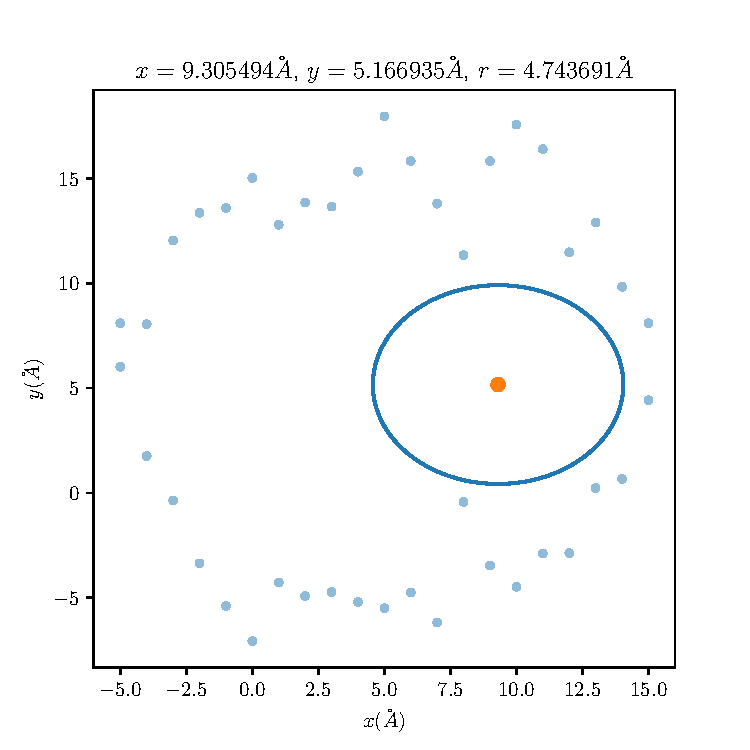
\includegraphics{canal_ionico_1.pdf}
		\caption{Circulo de mayor radio en el canal ionico encontrado en \texttt{Canal\_ionico.txt}.}
		\label{fig:canal}
	\end{figure}

	\begin{figure}
		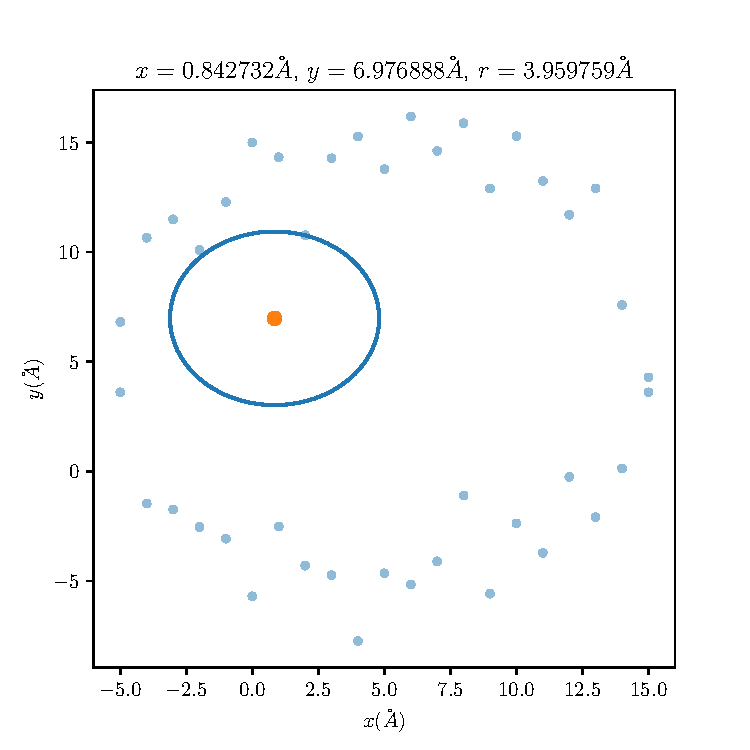
\includegraphics{canal_ionico_2.pdf}
		\caption{Circulo de mayor radio en el canal ionico encontrado en \texttt{Canal\_ionico1.txt}.}
		\label{fig:canal1}	
	\end{figure}

	\begin{figure}
		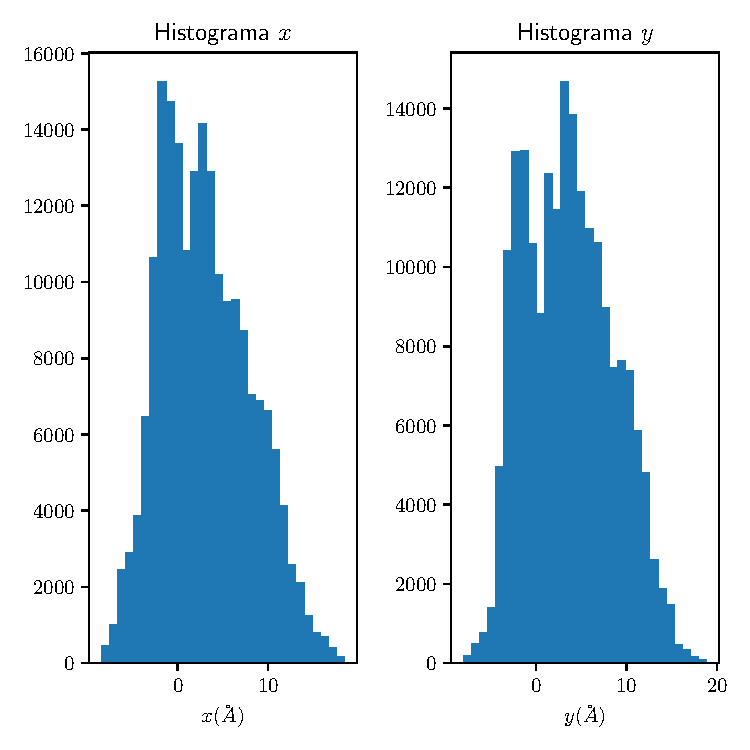
\includegraphics{histograma_1.pdf}
		\caption{Histograma del sampleo en el canal ionico encontrado en \texttt{Canal\_ionico.txt}.}
		\label{fig:hist}
	\end{figure}

	\begin{figure}
		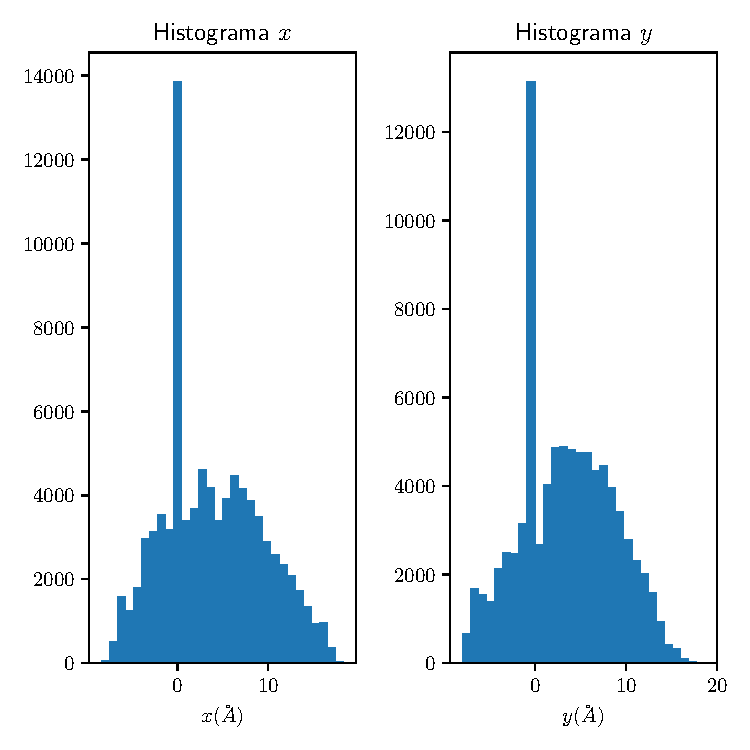
\includegraphics{histograma_2.pdf}
		\caption{Histograma del sampleo en el canal ionico encontrado en \texttt{Canal\_ionico1.txt}.}
		\label{fig:hist2}
	\end{figure}

Para la carga de un circuito $RC$ se utiliz\'o el sampleo en \ref{fig:hist3}. Este permiti\'o comparar distintos parametros generando \ref{fig:verosimilitud}. El ajuste final se muestra en \ref{fig:ajuste}.

	\begin{figure}
		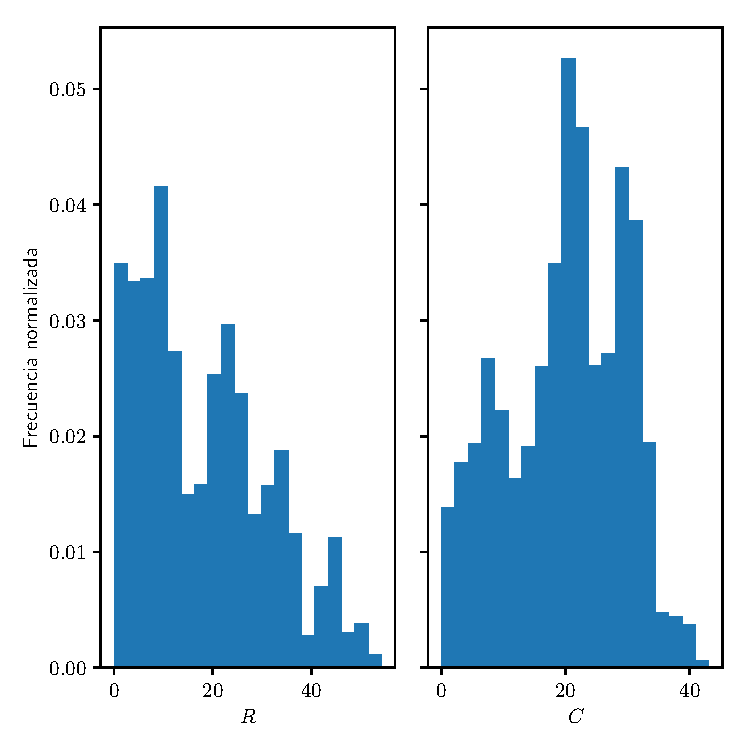
\includegraphics{histograma_3.pdf}
		\caption{Histograma del sampleo de resistencias y capacitancias.}
		\label{fig:hist3}
	\end{figure}

	\begin{figure}
		\includegraphics{verosimilitud.pdf}
		\caption{Comportamiento de parametros con respecto a la funci\'on de verosimilitud.}
		\label{fig:verosimilitud}
	\end{figure}

	\begin{figure} 
		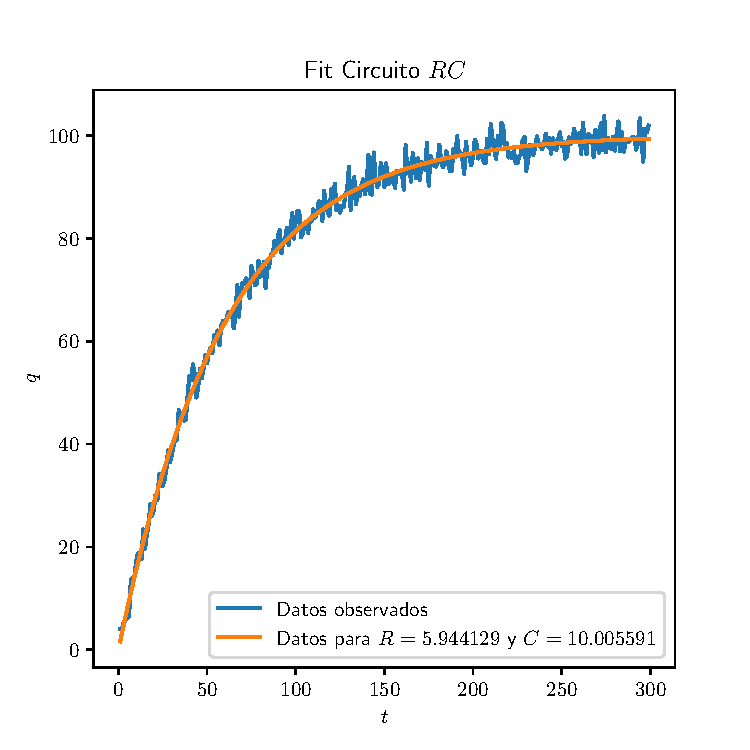
\includegraphics{best_fit.pdf}
		\caption{Ajuste de la carga de un circuito $RC$}
		\label{fig:ajuste}
	\end{figure}

\end{document}
